\chapter{Especificação de Requisitos}

\paragraph{}

\section{Requisitos Funcionais}

\subsection{Actores}

\subsubsection{Coordenador}

\subsubsection{Docente}

\subsubsection{Aluno}



\subsection{Casos de Uso}

\subsubsection{Gerir Inscrição em Momento de Avaliação}
	\textbf{Pré-Condições}\\
	O utilizador deve estar logado no sistema\\
	\textbf{Actores}\\
	Aluno\\
	\textbf{Cenário Principal}\\
	\textbf{Extensões ou Variações}\\

\subsubsection{Visualizar Momento de Avaliação}
	\textbf{Pré-Condições}\\
	O utilizador deve estar logado no sistema\\
	\textbf{Actores}\\
	Aluno, Coordenador e Docente\\
	\textbf{Cenário Principal}\\
	\textbf{Extensões ou Variações}\\

\subsubsection{Gerir Momento de Avaliação}
	\textbf{Pré-Condições}\\
	O utilizador deve estar logado no sistema\\
	\textbf{Actores}\\
	Docente\\
	\textbf{Cenário Principal}\\
	\textbf{Extensões ou Variações}\\



\subsubsection{Validar Avaliações}
	\textbf{Pré-Condições}\\
	O utilizador deve estar logado no sistema\\
	\textbf{Actores}\\
	Coordenador\\
	\textbf{Cenário Principal}\\
	\textbf{Extensões ou Variações}\\

\subsection{Diagrama de Classes}
(Seitz, 2009) \cite{seitz09:_gray_hat_python}.

\subsection{Base de Dados}
O modelo físico da Base de Dados pode ser consultado na \prettyref{fig:modelofisico}
\begin{figure}[h]
\centering
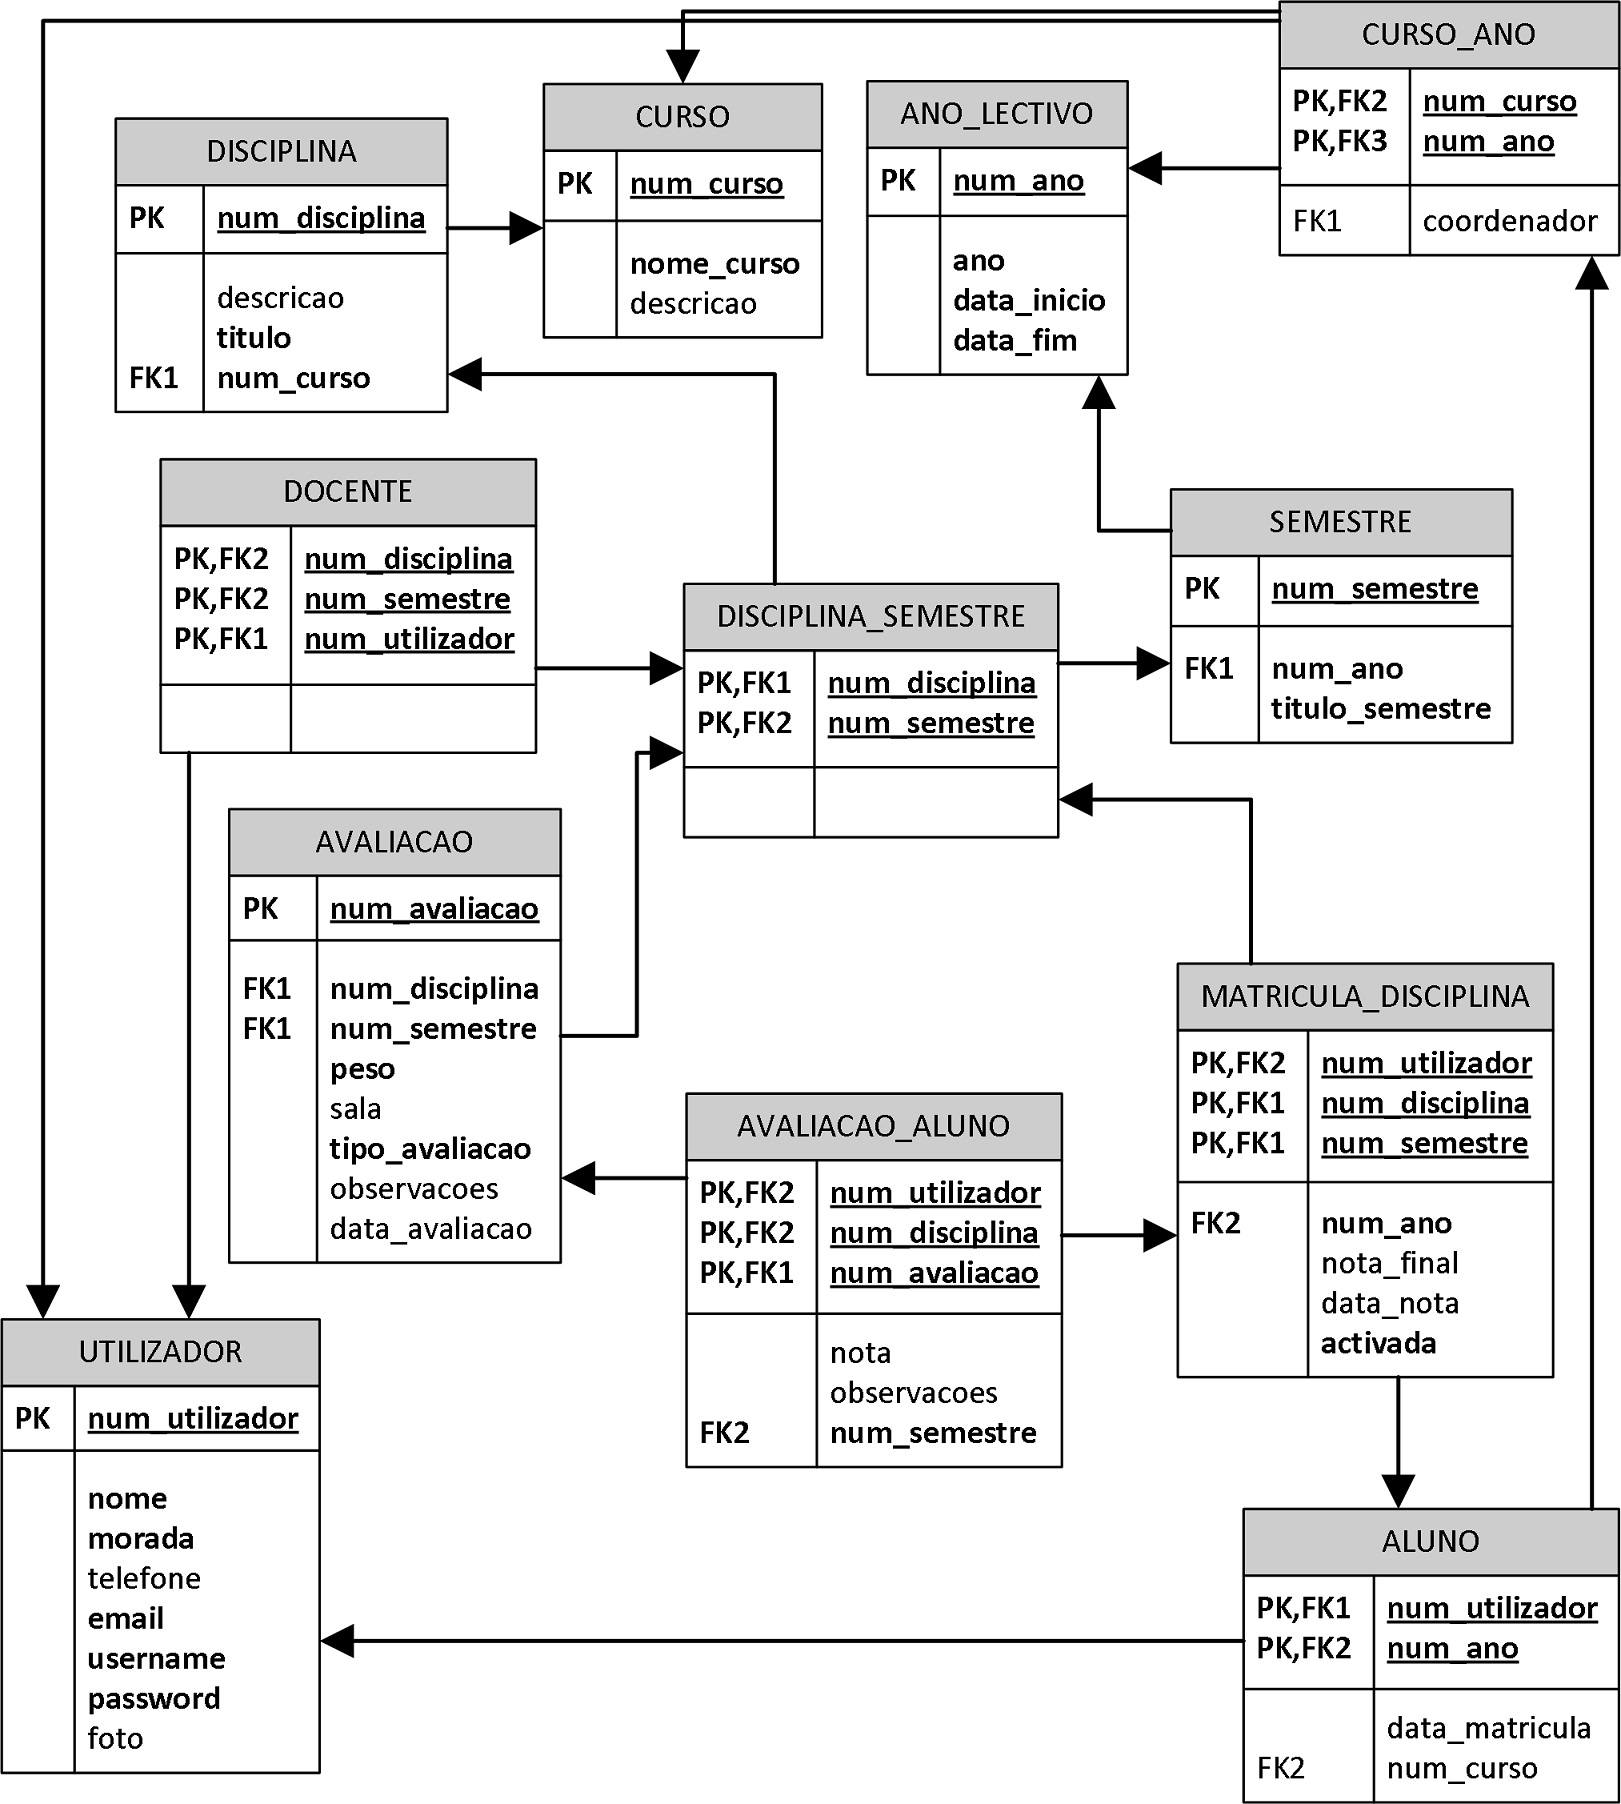
\includegraphics{imagens/modelofisico.jpg}
\caption{Base de Dados: Modelo Físico}
\label{fig:modelofisico}
\end{figure}
\section{Requisitos Não Funcionais}

\subsection{Requisitos do Produto}
O site a construir deverá respeitar os principais princípios e regras de Usabilidade e Acessibilidade, sendo que no último caso deverá respeitar o nível AA.
A autenticação dos membros deve ser efectuada através de sessões seguras.

\subsection{Requisitos Organizacionais}
O site será implementado em duas linguagens, PHP e ASP.NET utilizando bases de dados mySQL. Na versão PHP irão ser utilizados os API\'s jQuery e Smarty 

